\section{Using Tonemapping to Display the Entire Dynamic Range}\label{sec:toma}

To map the high dynamic range image to the eight bit values displayable by a
typical screen, I used the algorithm from \cite{dmac03}. This consists of
several steps.

I first converted the image to the CIE XYZ colorspace. For this,
I used the values provided at \cite{wik16}. Subsequently, I calculated the
maximum luminance (Y-value) in the image. I then used equation (4) from
\cite{dmac03} to calculate the luminance at each value. While I initally
expected to only have to do this with the Y-values, this did not produce useful
results. However, applying the same equation to the X and Z values resulted in
pleasing images, that preserved detail from the entire dynamic range. The
result is converted back to the RGB colorspace.

\cite{dmac03} suggest using gamma correction on the resulting image. I did
implement this; however, I did not notice an improvement in the image.
Unfortunately, the saturation in the tonemapped images seems quite low in
bright areas. In figure \ref{fig:toma}, three scenes can be seen,
after this algorithm has been used on their photographs.

\begin{figure}[ht]
  \centering
  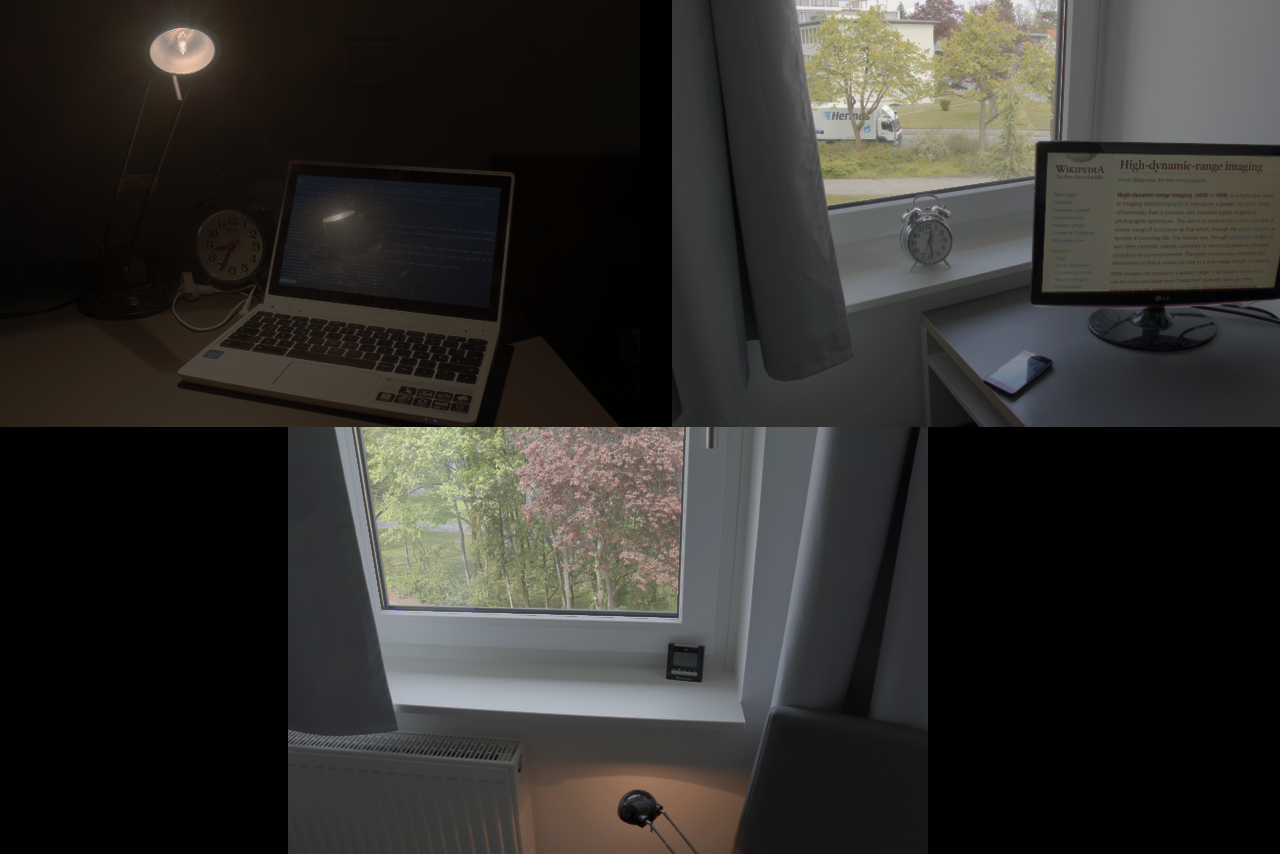
\includegraphics[width=\textwidth]{toma.png}
  \caption{The tonemapped images. Note that the image on the top left is quite
  dark - this is because of the extremely high intensities produced by the
  lightbulb being part of the image. However, it is also quite apparent that
  details of all intensities are preserved, as evidenced by the shading inside
  the lampshade}
  \label{fig:toma}
\end{figure}
